\chapter{Disoluciones y solubilidad}\label{ch:g6:solutions-and-solubility}

Se abre una botella de agua con gas: un silbido, y una nube de burbujas
diminutas sube de la nada. Un segundo antes el agua parecía
perfectamente transparente y, sin embargo, llevaba todo el tiempo un gas
disuelto. Los sólidos se \omterm{def:g2:mixing-and-dissolving:dissolve}{disuelven}, los líquidos se \omterm{def:g2:mixing-and-dissolving:dissolve}{disuelven}, y los
gases también, pero nunca sin límite. Este capítulo pone nombre a las
partes de una disolución y mide cuánta cantidad de una sustancia puede
admitir un líquido.

\begin{recall}
Un sólido que se \omterm{def:g2:mixing-and-dissolving:dissolve}{disuelve} en agua desaparece de la vista y deja el
líquido transparente; ese líquido transparente es una disolución, y lo
que se ha disuelto sigue en ella (\cref{ch:g2:mixing-and-dissolving}).
Una disolución es una \omterm{def:g6:pure-substances-and-mixtures:homogeneous}{mezcla homogénea} de \omterm{def:g6:pure-substances-and-mixtures:species}{especies químicas}
(\cref{ch:g6:pure-substances-and-mixtures}). \omterm{def:g3:separating-mixtures:evaporate}{Evaporando} el agua se
recupera el sólido disuelto (\cref{ch:g3:separating-mixtures}).
\end{recall}

\begin{omfigure}
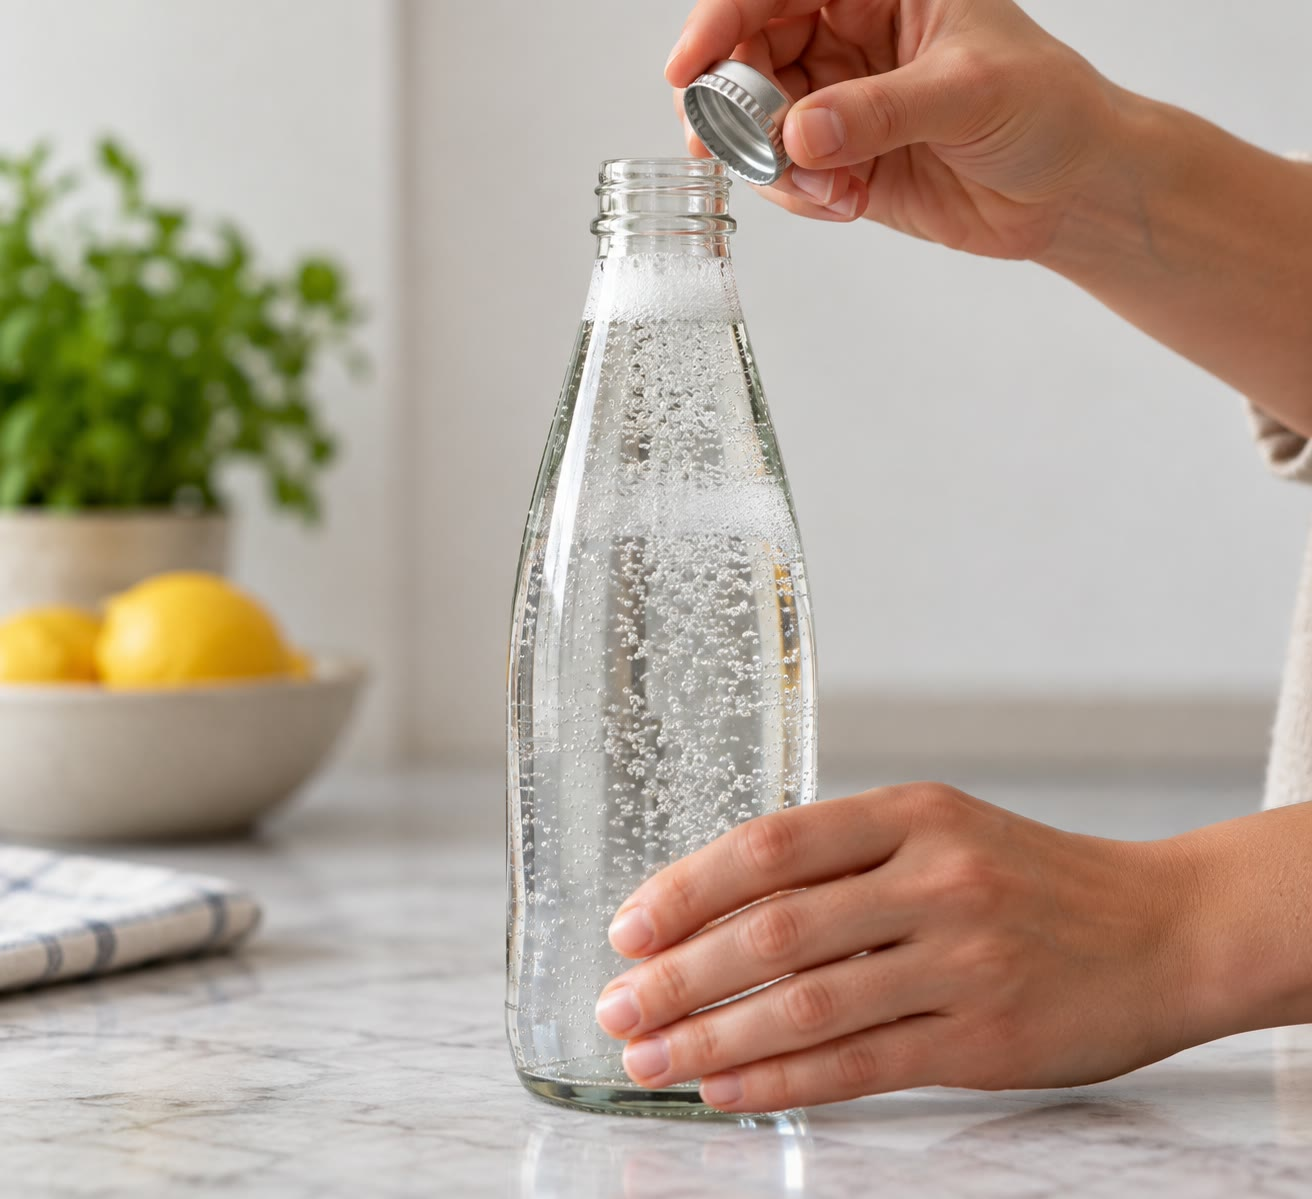
\includegraphics[width=0.5\linewidth]{images/book1/ai/g6-fizzy-water.jpg}

{\small Al abrir una botella de agua con gas, el gas disuelto sale en
forma de burbujas.}
\end{omfigure}

\section{Soluto y disolvente}

\begin{definition}[Soluto, disolvente, disolución acuosa]\label{def:g6:solutions-and-solubility:solute}
En una disolución, la sustancia que se \omterm{def:g2:mixing-and-dissolving:dissolve}{disuelve} es el
\emph{soluto}\index{soluto}, y el líquido en el que se \omterm{def:g2:mixing-and-dissolving:dissolve}{disuelve} es el
\emph{disolvente}\index{disolvente}. Cuando el disolvente es el agua, la
disolución es una \emph{disolución acuosa}\index{disolucion acuosa@disolución acuosa}.
\end{definition}

\begin{example}[Disolventes distintos del agua]\label{ex:g6:solutions-and-solubility:solvents}
El agua es el \omterm{def:g6:solutions-and-solubility:solute}{disolvente} más corriente, pero no el único. El esmalte de
uñas no se \omterm{def:g2:mixing-and-dissolving:dissolve}{disuelve} en agua; se \omterm{def:g2:mixing-and-dissolving:dissolve}{disuelve} en propanona (acetona), el
\omterm{def:g6:solutions-and-solubility:solute}{disolvente} del quitaesmalte. La grasa y la pintura al óleo se \omterm{def:g2:mixing-and-dissolving:dissolve}{disuelven}
en aguarrás. Muchos medicamentos se \omterm{def:g2:mixing-and-dissolving:dissolve}{disuelven} en etanol. Una disolución
puede tener varios \omterm{def:g6:solutions-and-solubility:solute}{solutos}: el agua del mar contiene sal disuelta y
muchas otras sustancias.
\end{example}

\begin{safety}{\ghs{GHS02}\ghs{GHS07}}
% ledger: ghs:acetone
Propanona (acetona): líquido y vapores muy inflamables (GHS02); irrita
los ojos y sus vapores pueden provocar somnolencia o vértigo (GHS07). Se
usa en una sala ventilada, lejos de cualquier llama.
\end{safety}

\begin{proposition}[Las masas se suman]\label{prop:g6:solutions-and-solubility:mass}
La masa de una disolución es la masa del \omterm{def:g6:solutions-and-solubility:solute}{disolvente} más la masa del
\omterm{def:g6:solutions-and-solubility:solute}{soluto} disuelto: cuando un sólido se \omterm{def:g2:mixing-and-dissolving:dissolve}{disuelve} no se pierde nada, aunque
ya no se vea.
\end{proposition}

\begin{omfigure}
\begin{tikzpicture}[font=\small, scale=1.15]
  \pic[transform shape] at (0,0) {balance};
  \pic[transform shape] at (0,0.8) {beaker={0.5}{omWater!80}};
  \node[anchor=north, align=center] at (0,-0.1) {\qty{100}{g} de agua};
  \node at (1.85,1.3) {$+$};
  \pic[transform shape] at (3.5,0) {balance};
  \fill[white, draw=black!45] (3.0,0.8) rectangle (4.0,0.9);
  \fill[white, draw=black!45] (3.15,0.9) -- (3.85,0.9) -- (3.5,1.2) -- cycle;
  \node[anchor=north, align=center] at (3.5,-0.1) {\qty{10}{g} de azúcar};
  \draw[->, thick, omProp] (4.9,1.2) -- (6.0,1.2) node[midway, above, text=black]
    {remover};
  \pic[transform shape] at (7.4,0) {balance};
  \pic[transform shape] at (7.4,0.8) {beaker={0.52}{omWater!80}};
  \node[anchor=north, align=center] at (7.4,-0.1) {\qty{110}{g} de agua con azúcar};
\end{tikzpicture}

{\small Al \omterm{def:g2:mixing-and-dissolving:dissolve}{disolver} \qty{10}{g} de azúcar en \qty{100}{g} de agua se
obtienen \qty{110}{g} de disolución (sin contar la masa del vaso).}
\end{omfigure}

\section{Saturación y solubilidad}

\begin{definition}[Disolución saturada]\label{def:g6:solutions-and-solubility:saturated}
Una disolución es una \emph{disolución saturada}\index{disolucion saturada@disolución saturada}
cuando ya no puede \omterm{def:g2:mixing-and-dissolving:dissolve}{disolver} más \omterm{def:g6:solutions-and-solubility:solute}{soluto}: todo el \omterm{def:g6:solutions-and-solubility:solute}{soluto} que se añade se
queda en el fondo, sin \omterm{def:g2:mixing-and-dissolving:dissolve}{disolver}, por mucho que removamos.
\end{definition}

\begin{definition}[Solubilidad]\label{def:g6:solutions-and-solubility:solubility}
La \emph{solubilidad}\index{solubilidad} de un \omterm{def:g6:solutions-and-solubility:solute}{soluto} en un \omterm{def:g6:solutions-and-solubility:solute}{disolvente}
es la mayor masa de \omterm{def:g6:solutions-and-solubility:solute}{soluto} que puede \omterm{def:g2:mixing-and-dissolving:dissolve}{disolver} una cantidad dada de
\omterm{def:g6:solutions-and-solubility:solute}{disolvente}, a una temperatura dada. Para un sólido en agua se suele dar
en gramos por litro (o por kilogramo) de agua.
\end{definition}

\begin{proposition}[Algunas solubilidades en agua]\label{prop:g6:solutions-and-solubility:values}
% ledger: sol:NaCl, sol:sucrose, sol:CO2, sol:O2 (O2: 31 mL/L, 31/24.0 x 32 = 0.041 g/L at 20 C)
Las \omterm{def:g6:solutions-and-solubility:solubility}{solubilidades} medidas en agua son enormemente distintas:
\begin{center}
\small
\begin{tabular}{lll}
\hline
\omterm{def:g6:solutions-and-solubility:solute}{soluto} & \omterm{def:g6:solutions-and-solubility:solubility}{solubilidad} en agua & condiciones \\
\hline
azúcar (sacarosa) & unos \qty{2000}{g} por litro de agua & temperatura ambiente \\
sal (cloruro de sodio) & \qty{360}{g} por kilogramo de agua & \qty{25}{\celsius} \\
dióxido de carbono & unos \qty{1.5}{g} por litro & \qty{25}{\celsius}, bajo el gas \\
oxígeno & unos \qty{0.04}{g} por litro & \qty{20}{\celsius}, bajo el gas \\
arena, tiza & prácticamente nula & --- \\
\hline
\end{tabular}
\end{center}
Un litro de agua puede \omterm{def:g2:mixing-and-dissolving:dissolve}{disolver} más de su propia masa de azúcar, pero
ni siquiera medio gramo de oxígeno.
\end{proposition}

\begin{method}[¿Se disolverá todo?]\label{met:g6:solutions-and-solubility:will-it}
Para saber si una masa $m$ de \omterm{def:g6:solutions-and-solubility:solute}{soluto} se \omterm{def:g2:mixing-and-dissolving:dissolve}{disuelve} por completo en un
volumen de agua:
\begin{enumerate}
  \item buscar la \omterm{def:g6:solutions-and-solubility:solubility}{solubilidad} del \omterm{def:g6:solutions-and-solubility:solute}{soluto} (en g por litro de agua);
  \item calcular la mayor masa que puede \omterm{def:g2:mixing-and-dissolving:dissolve}{disolver} ese volumen de agua;
  \item compararla con $m$: si $m$ es menor, todo se \omterm{def:g2:mixing-and-dissolving:dissolve}{disuelve}; si $m$ es
        mayor, la disolución queda saturada y el resto se queda en el
        fondo.
\end{enumerate}
\end{method}

\begin{example}[Sal en un vaso]\label{ex:g6:solutions-and-solubility:glass}
% ledger: sol:NaCl
¿Se pueden \omterm{def:g2:mixing-and-dissolving:dissolve}{disolver} \qty{50}{g} de sal en \qty{200}{mL} de agua (unos
\qty{200}{g})? Un kilogramo de agua \omterm{def:g2:mixing-and-dissolving:dissolve}{disuelve} como mucho \qty{360}{g}
de sal, así que \qty{200}{g} de agua \omterm{def:g2:mixing-and-dissolving:dissolve}{disuelven} como mucho $360 \times
\frac{200}{1000} = \qty{72}{g}$. Como $50 < 72$, toda la sal se
\omterm{def:g2:mixing-and-dissolving:dissolve}{disuelve}.
\end{example}

\begin{omfigure}
\begin{tikzpicture}[font=\small, scale=1.15]
  \pic[transform shape] at (0,0) {beaker={0.6}{omWater!80}};
  \node[anchor=north, align=center] at (0,-0.15) {un poco de sal:\\ todo disuelto};
  \pic[transform shape] at (3.2,0) {beaker={0.6}{omWater!80}};
  \node[anchor=north, align=center] at (3.2,-0.15) {más sal:\\ justo saturada};
  \pic[transform shape] at (6.4,0) {beaker={0.6}{omWater!80}};
  \fill[black!12, draw=black!50] (5.7,0) -- (7.1,0) -- (6.9,0.2) -- (5.9,0.2) -- cycle;
  \foreach \x in {5.85,6.05,6.25,6.45,6.65,6.85} \fill[black!45] (\x,0.09) circle (0.03);
  \node[anchor=north, align=center] at (6.4,-0.15) {demasiada sal:\\ el resto queda sin disolver};
\end{tikzpicture}

{\small Se añade cada vez más sal a la misma agua. Una vez saturada la
disolución, la sal que sobra se queda en el fondo.}
\end{omfigure}

\begin{inthelab}[Saturar agua con sal]
El profesor añade sal a \qty{100}{mL} de agua, cucharada a cucharada,
removiendo bien después de cada una. Las primeras cucharadas
desaparecen; luego una cucharada ya no se \omterm{def:g2:mixing-and-dissolving:dissolve}{disuelve} del todo y unos
granos blancos se quedan en el fondo: la disolución está saturada. Al
pesar la sal usada se ve que se han disuelto unos \qty{36}{g}.
\end{inthelab}

\section{Líquidos miscibles e inmiscibles}

\begin{definition}[Líquidos miscibles e inmiscibles]\label{def:g6:solutions-and-solubility:miscible}
Dos líquidos son \emph{miscibles}\index{miscibles} cuando, \omterm{def:g2:mixing-and-dissolving:mix}{mezclados},
dan un único líquido homogéneo. Son
\emph{inmiscibles}\index{inmiscibles} cuando se separan en dos capas,
con la más ligera arriba.
\end{definition}

\begin{example}[Agua con etanol, agua con aceite]\label{ex:g6:solutions-and-solubility:liquids}
El agua y el etanol son \omterm{def:g6:solutions-and-solubility:miscible}{miscibles}: agitados juntos, dan un único líquido
transparente. El agua y el aceite son \omterm{def:g6:solutions-and-solubility:miscible}{inmiscibles}: por mucho que se
agiten, el aceite vuelve a subir y flota sobre el agua formando una capa
aparte. En un tarro de vinagreta, el aceite flota sobre el vinagre, que
es sobre todo agua.
\end{example}

\begin{omfigure}
\begin{tikzpicture}[font=\small, scale=1.3]
  \pic[transform shape] at (0,0) {testtube={0.6}{omWater!80}};
  \node[anchor=north, align=center] at (0,-0.15) {agua + etanol:\\ una capa};
  \pic[transform shape] at (3,0) {testtube={0.65}{yellow!55!orange!60}};
  \begin{scope}
    \clip (2.75,3) -- (2.75,0.25) arc[start angle=180, end angle=360, radius=0.25]
      -- (3.25,3) -- cycle;
    \fill[omWater!80] (2.7,0) rectangle (3.3,1.1);
  \end{scope}
  \draw[omGlass, line width=0.7pt] (2.75,3) -- (2.75,0.25) arc[start angle=180,
    end angle=360, radius=0.25] -- (3.25,3);
  \draw[<-, omProp, thick] (3.3,1.55) -- (4.1,1.75) node[right, text=black] {aceite};
  \draw[<-, omProp, thick] (3.3,0.6) -- (4.1,0.6) node[right, text=black] {agua};
  \node[anchor=north, align=center] at (3,-0.15) {agua + aceite:\\ dos capas};
\end{tikzpicture}

{\small Los líquidos \omterm{def:g6:solutions-and-solubility:miscible}{miscibles} dan una capa; los \omterm{def:g6:solutions-and-solubility:miscible}{inmiscibles}, dos.}
\end{omfigure}

\begin{omfigure}
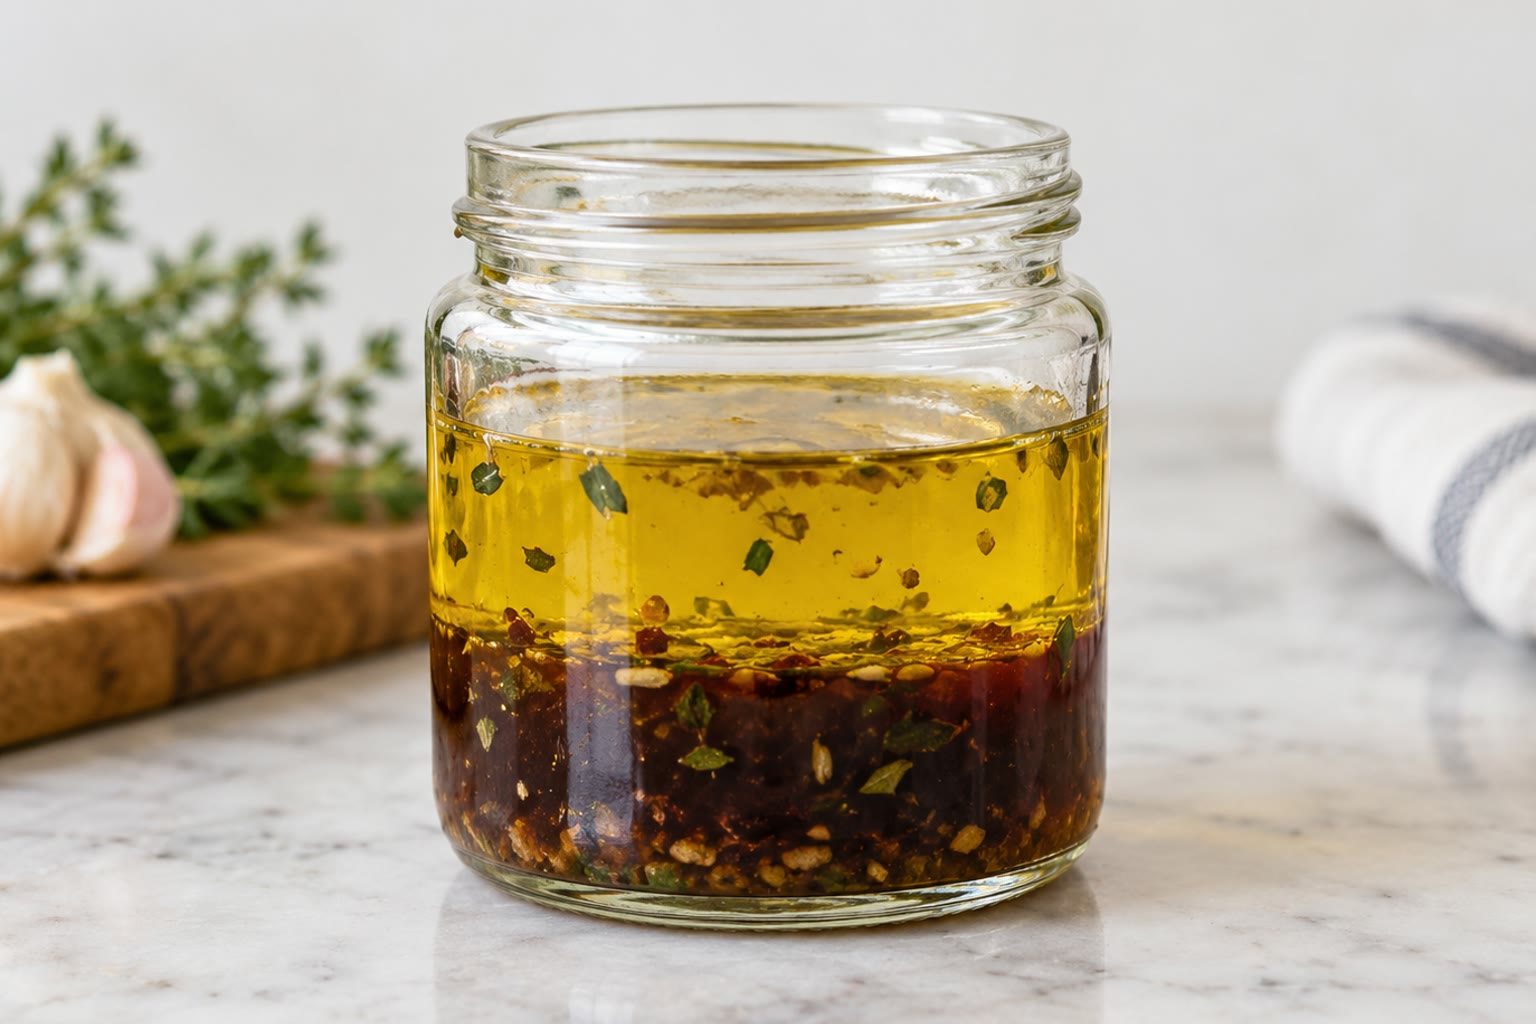
\includegraphics[width=0.45\linewidth]{images/book1/ai/g6-vinaigrette.jpg}

{\small Una vinagreta: el aceite y el vinagre son \omterm{def:g6:solutions-and-solubility:miscible}{inmiscibles}.}
\end{omfigure}

\section{Los gases también se disuelven}

\begin{proposition}[Gases disueltos]\label{prop:g6:solutions-and-solubility:gases}
Los gases se \omterm{def:g2:mixing-and-dissolving:dissolve}{disuelven} en el agua, un poco. Las bebidas con gas se
fabrican \omterm{def:g2:mixing-and-dissolving:dissolve}{disolviendo} en ellas dióxido de carbono a presión en una
botella cerrada; al abrir la botella, parte del gas vuelve a salir en
forma de burbujas. El agua en contacto con el \omterm{def:g4:air-a-mixture-of-gases:air}{aire} contiene algo de
oxígeno disuelto, que los peces toman por las branquias. Un gas se
\omterm{def:g2:mixing-and-dissolving:dissolve}{disuelve} menos en agua templada que en agua fría: una bebida con gas
templada se queda sin gas antes.
\end{proposition}

\begin{example}[Los océanos y el dióxido de carbono]\label{ex:g6:solutions-and-solubility:oceans}
Los océanos están en contacto con el \omterm{def:g4:air-a-mixture-of-gases:air}{aire} en dos terceras partes de la
superficie de la Tierra. El dióxido de carbono del \omterm{def:g4:air-a-mixture-of-gases:air}{aire} se \omterm{def:g2:mixing-and-dissolving:dissolve}{disuelve} en
ellos, de modo que los océanos absorben parte del dióxido de carbono que
las personas liberan al \omterm{def:g4:air-a-mixture-of-gases:air}{aire}.
\end{example}

\begin{omfigure}
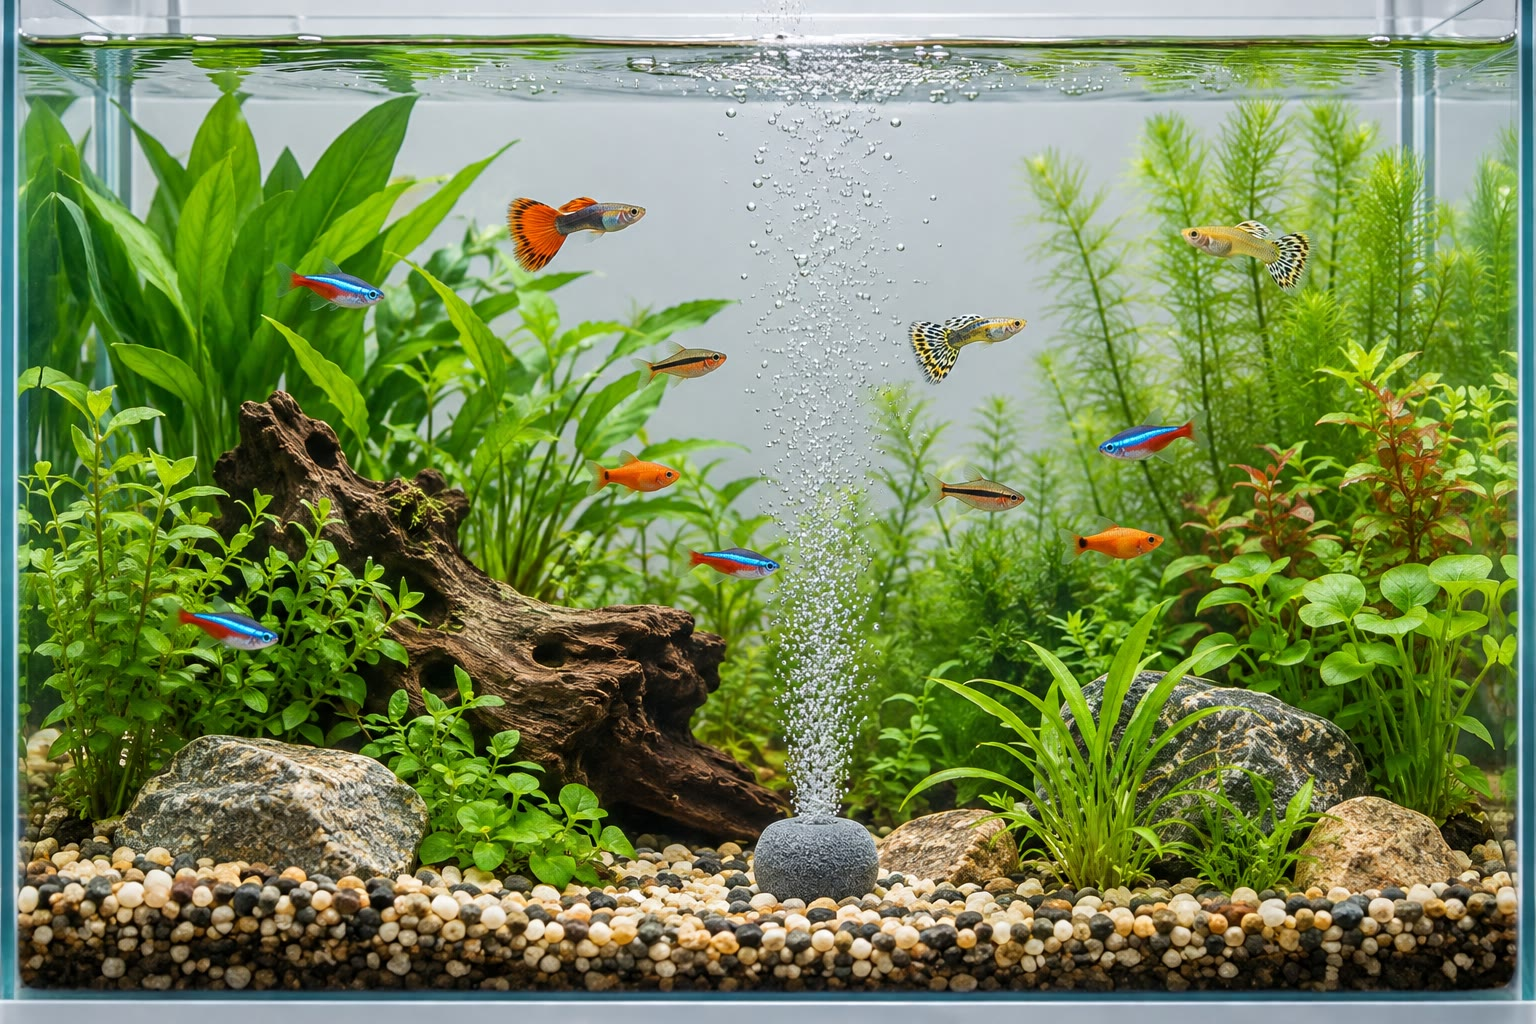
\includegraphics[width=0.5\linewidth]{images/book1/ai/g6-fish-tank.jpg}

{\small Un acuario: las burbujas de \omterm{def:g4:air-a-mixture-of-gases:air}{aire} mantienen el agua provista de
oxígeno disuelto para los peces.}
\end{omfigure}

\section{Ejercicios}

\begin{exercise}[$\star$]\label{exo:g6:solutions-and-solubility:1}
En el agua con azúcar, nombra el \omterm{def:g6:solutions-and-solubility:solute}{soluto} y el \omterm{def:g6:solutions-and-solubility:solute}{disolvente}. ¿Es una
\omterm{def:g6:solutions-and-solubility:solute}{disolución acuosa}?
\end{exercise}

\begin{exercise}[$\star$]\label{exo:g6:solutions-and-solubility:2}
¿Qué es una \omterm{def:g6:solutions-and-solubility:saturated}{disolución saturada}? ¿Cómo se ve que una disolución está
saturada?
\end{exercise}

\begin{exercise}[$\star$]\label{exo:g6:solutions-and-solubility:3}
Se \omterm{def:g2:mixing-and-dissolving:dissolve}{disuelven} \qty{20}{g} de sal en \qty{250}{g} de agua. ¿Cuál es la
masa de la disolución?
\end{exercise}

\begin{exercise}[$\star$]\label{exo:g6:solutions-and-solubility:4}
¿\omterm{def:g6:solutions-and-solubility:miscible}{Miscible} o \omterm{def:g6:solutions-and-solubility:miscible}{inmiscible} con el agua: el etanol, el aceite de cocina, el
vinagre?
\end{exercise}

\begin{exercise}[$\star$]\label{exo:g6:solutions-and-solubility:5}
Nombra el \omterm{def:g6:solutions-and-solubility:solute}{disolvente} del quitaesmalte y da el significado de sus dos
pictogramas.
\end{exercise}

\begin{exercise}[$\star\star$]\label{exo:g6:solutions-and-solubility:6}
Con la \omterm{def:g6:solutions-and-solubility:solubility}{solubilidad} de la sal, halla la mayor masa de sal que pueden
\omterm{def:g2:mixing-and-dissolving:dissolve}{disolver} \qty{500}{g} de agua a \qty{25}{\celsius}.
\end{exercise}

\begin{exercise}[$\star\star$]\label{exo:g6:solutions-and-solubility:7}
Se remueven \qty{80}{g} de sal en \qty{200}{g} de agua a
\qty{25}{\celsius}. ¿Se \omterm{def:g2:mixing-and-dissolving:dissolve}{disuelve} toda? Si no, ¿qué masa se queda en el
fondo?
\end{exercise}

\begin{exercise}[$\star\star$]\label{exo:g6:solutions-and-solubility:8}
Se \omterm{def:g2:mixing-and-dissolving:dissolve}{disuelven} \qty{25}{g} de azúcar en \qty{225}{g} de agua. ¿Qué
porcentaje de la masa de la disolución es azúcar?
\end{exercise}

\begin{exercise}[$\star\star$]\label{exo:g6:solutions-and-solubility:9}
Mira la figura de los tres vasos de agua con sal. ¿En qué vaso podría
\omterm{def:g2:mixing-and-dissolving:dissolve}{disolverse} todavía más sal?
\end{exercise}

\begin{exercise}[$\star\star$]\label{exo:g6:solutions-and-solubility:10}
¿Por qué una botella de agua con gas burbujea al abrirla, y no antes?
\end{exercise}

\begin{exercise}[$\star\star\star$]\label{exo:g6:solutions-and-solubility:11}
Un litro de agua puede \omterm{def:g2:mixing-and-dissolving:dissolve}{disolver} unos \qty{2000}{g} de azúcar, pero solo
unos \qty{0.04}{g} de oxígeno. ¿Cuántas veces más azúcar que oxígeno es
eso?
\end{exercise}

\begin{exercise}[$\star\star\star$]\label{exo:g6:solutions-and-solubility:12}
En verano, el agua de un estanque se calienta y los peces suben a la
superficie a tragar \omterm{def:g4:air-a-mixture-of-gases:air}{aire}. Usa este capítulo para explicar por qué.
\end{exercise}

\section{Problema: La salmuera del quesero}

\begin{problem}[{Problema de fin de semana --- un baño de agua saturada
de sal para los quesos, y lo que le hace el calor del verano}]
\label{pb:g6:solutions-and-solubility:1}
% ledger: sol:NaCl (360 g per kg of water; 1 L of water taken as 1 kg)
Muchos quesos se sumergen unas horas en un baño de salmuera: agua
saturada de sal. Un quesero llena un depósito con \qty{20}{L} de agua
(\qty{20}{kg}) y añade sal hasta que una parte se queda sin \omterm{def:g2:mixing-and-dissolving:dissolve}{disolver} en
el fondo. Toma como \omterm{def:g6:solutions-and-solubility:solubility}{solubilidad} de la sal \qty{360}{g} por kilogramo de
agua.

\medskip
\noindent\textbf{Parte I --- Las palabras.}
\begin{enumerate}
  \item En la salmuera, ¿cuál es el \omterm{def:g6:solutions-and-solubility:solute}{soluto} y cuál el \omterm{def:g6:solutions-and-solubility:solute}{disolvente}?
  \item ¿Qué significa ``saturada'' en el caso de la salmuera?
  \item ¿Por qué añade el quesero sal hasta que queda un poco en el
        fondo?
\end{enumerate}

\medskip
\noindent\textbf{Parte II --- Preparar la salmuera.}
\begin{enumerate}[resume]
  \item ¿Qué masa de sal se \omterm{def:g2:mixing-and-dissolving:dissolve}{disuelve} en los \qty{20}{kg} de agua?
  \item ¿Cuál es la masa de la salmuera (sin la sal no disuelta)?
  \item ¿Qué porcentaje de la masa de la salmuera es sal? Redondea al
        número entero más próximo.
  \item Un día solo se añaden \qty{5}{kg} de sal. ¿Está saturada la
        salmuera? ¿Cuánta sal más podría \omterm{def:g2:mixing-and-dissolving:dissolve}{disolver}?
\end{enumerate}

\medskip
\noindent\textbf{Parte III --- Un verano caluroso.}
Durante una semana de calor se \omterm{def:g3:separating-mixtures:evaporate}{evaporan} \qty{5}{L} (\qty{5}{kg}) de agua
de la salmuera saturada de la parte II, sin que se pierda nada de sal.
\begin{enumerate}[resume]
  \item ¿Cuánta agua queda en el depósito?
  \item ¿Qué masa de sal puede seguir teniendo disuelta esta agua?
  \item ¿Qué le pasa a la sal que el agua restante no puede retener?
  \item ¿Cómo puede ver el quesero, a simple vista, que esto ha
        ocurrido?
  \item Calcula la masa de sal que ha cristalizado en el fondo del
        depósito.
\end{enumerate}
\end{problem}
